\chapter{Development Process}
\label{ch:development_process}

This chapter details the process of translating stakeholder needs into a functioning dashboard application. It covers prioritization of requirements, technology selection, planning, iterative development, and testing activities. It also reflects on practical choices made throughout development, supported by figures, diagrams, and code snippets.

\section{Defining Requirements}
\label{sec:def_req}

As outlined in \autoref{subsec:req_gathering}, the project’s requirements were shaped through a combination of assignment analysis, stakeholder dialogue, and iterative prototyping. This section presents how requirements evolved from an initial internal interpretation of the client’s brief, through stakeholder clarification, and were ultimately refined following feedback from prototype testing.

\subsection{Initial Requirements from Assignment Brief}
\label{subsec:req_from_brief}
The initial step in the requirement elicitation process involved a detailed analysis of the \textbf{\hyperref[app:headspin-brief]{assignment brief}}. This internal review helped clarify the project’s technical scope, overall purpose, and core expectations as defined by Headspin AS. Based on this document, a preliminary set of functional and non-functional requirements was defined.

These requirements focused on baseline dashboard capabilities such as website monitoring, status display, and per-website data. The goal at this stage was to obtain a high-level understanding of what the system should achieve.

\begin{table}[H]
\centering
\caption{Functional Requirements from Brief}
\label{tab:functional_reqs_brief}
\begin{tabular}{| l  |p{0.6\textwidth}  |l |} 
\hline
\textbf{Req ID} & \textbf{Requirement Title} & \textbf{Priority} \\
\hline
F.1 & Add, edit, and delete monitored websites via the GUI. & High \\ \hline 
F.2 & Set custom check intervals per site. & High \\ \hline 
F.3 & Display current HTTP status, last response time, and uptime history. & High \\ \hline 
F.4 & Check whether the website is truly up (not just HTTP status). & High \\ \hline 
F.5 & Trigger alerts and notifications via email or SMS. & Medium \\ \hline
F.6 & Support visual filters and sorting mechanisms. & Medium \\
\hline
\end{tabular}
\end{table}

\begin{table}[H]
    \centering
    \caption{Non-Functional Requirements from Brief}
    \label{tab:non_functional_reqs_brief}
    \begin{tabular}{| l  |p{0.6\textwidth}  |l |}
        \hline
        \textbf{Req ID} & \textbf{Requirement Title} & \textbf{Priority} \\
        \hline
        NF.1 & The system must support monitoring of multiple sites without delay. & High \\ \hline 
        NF.2 & The user should easily interpret website status changes. & High \\ \hline 
        NF.3 & The system should be user-friendly and intuitive. & High \\ \hline 
        NF.4 & The system must be maintainable and well-documented. & Medium \\ \hline
    \end{tabular}
\end{table}

\subsection{Stakeholder meeting}

To validate and expand upon the preliminary requirements, a clarification meeting was conducted with stakeholders at Headspin AS. This meeting revealed the presence of two key user groups with differing needs. Employees who regularly communicated with clients wanted historical uptime summaries they could show to clients, while internal developers highlighted the need for real-time data and efficient management of monitored websites.

The meeting clarified who the users of the dashboard application would be and led to several changes. Notably, personalization features such as user-specific dashboards and filtering options were added as requirements. 

\subsection{Prototyping}

To further verify the requirements gathered from the meeting with stakeholders at Headspin AS, a functional prototype of the dashboard was developed (See \ref{fig:proto_dash}). This prototype focused on core components such as a dashboard view,  website status cards, as well as basic navigation. The prototype also served as the foundation for early usability testing in \hyperref[subsec:user_testing]{user test 1}. 

\begin{figure}[H]
    \centering
    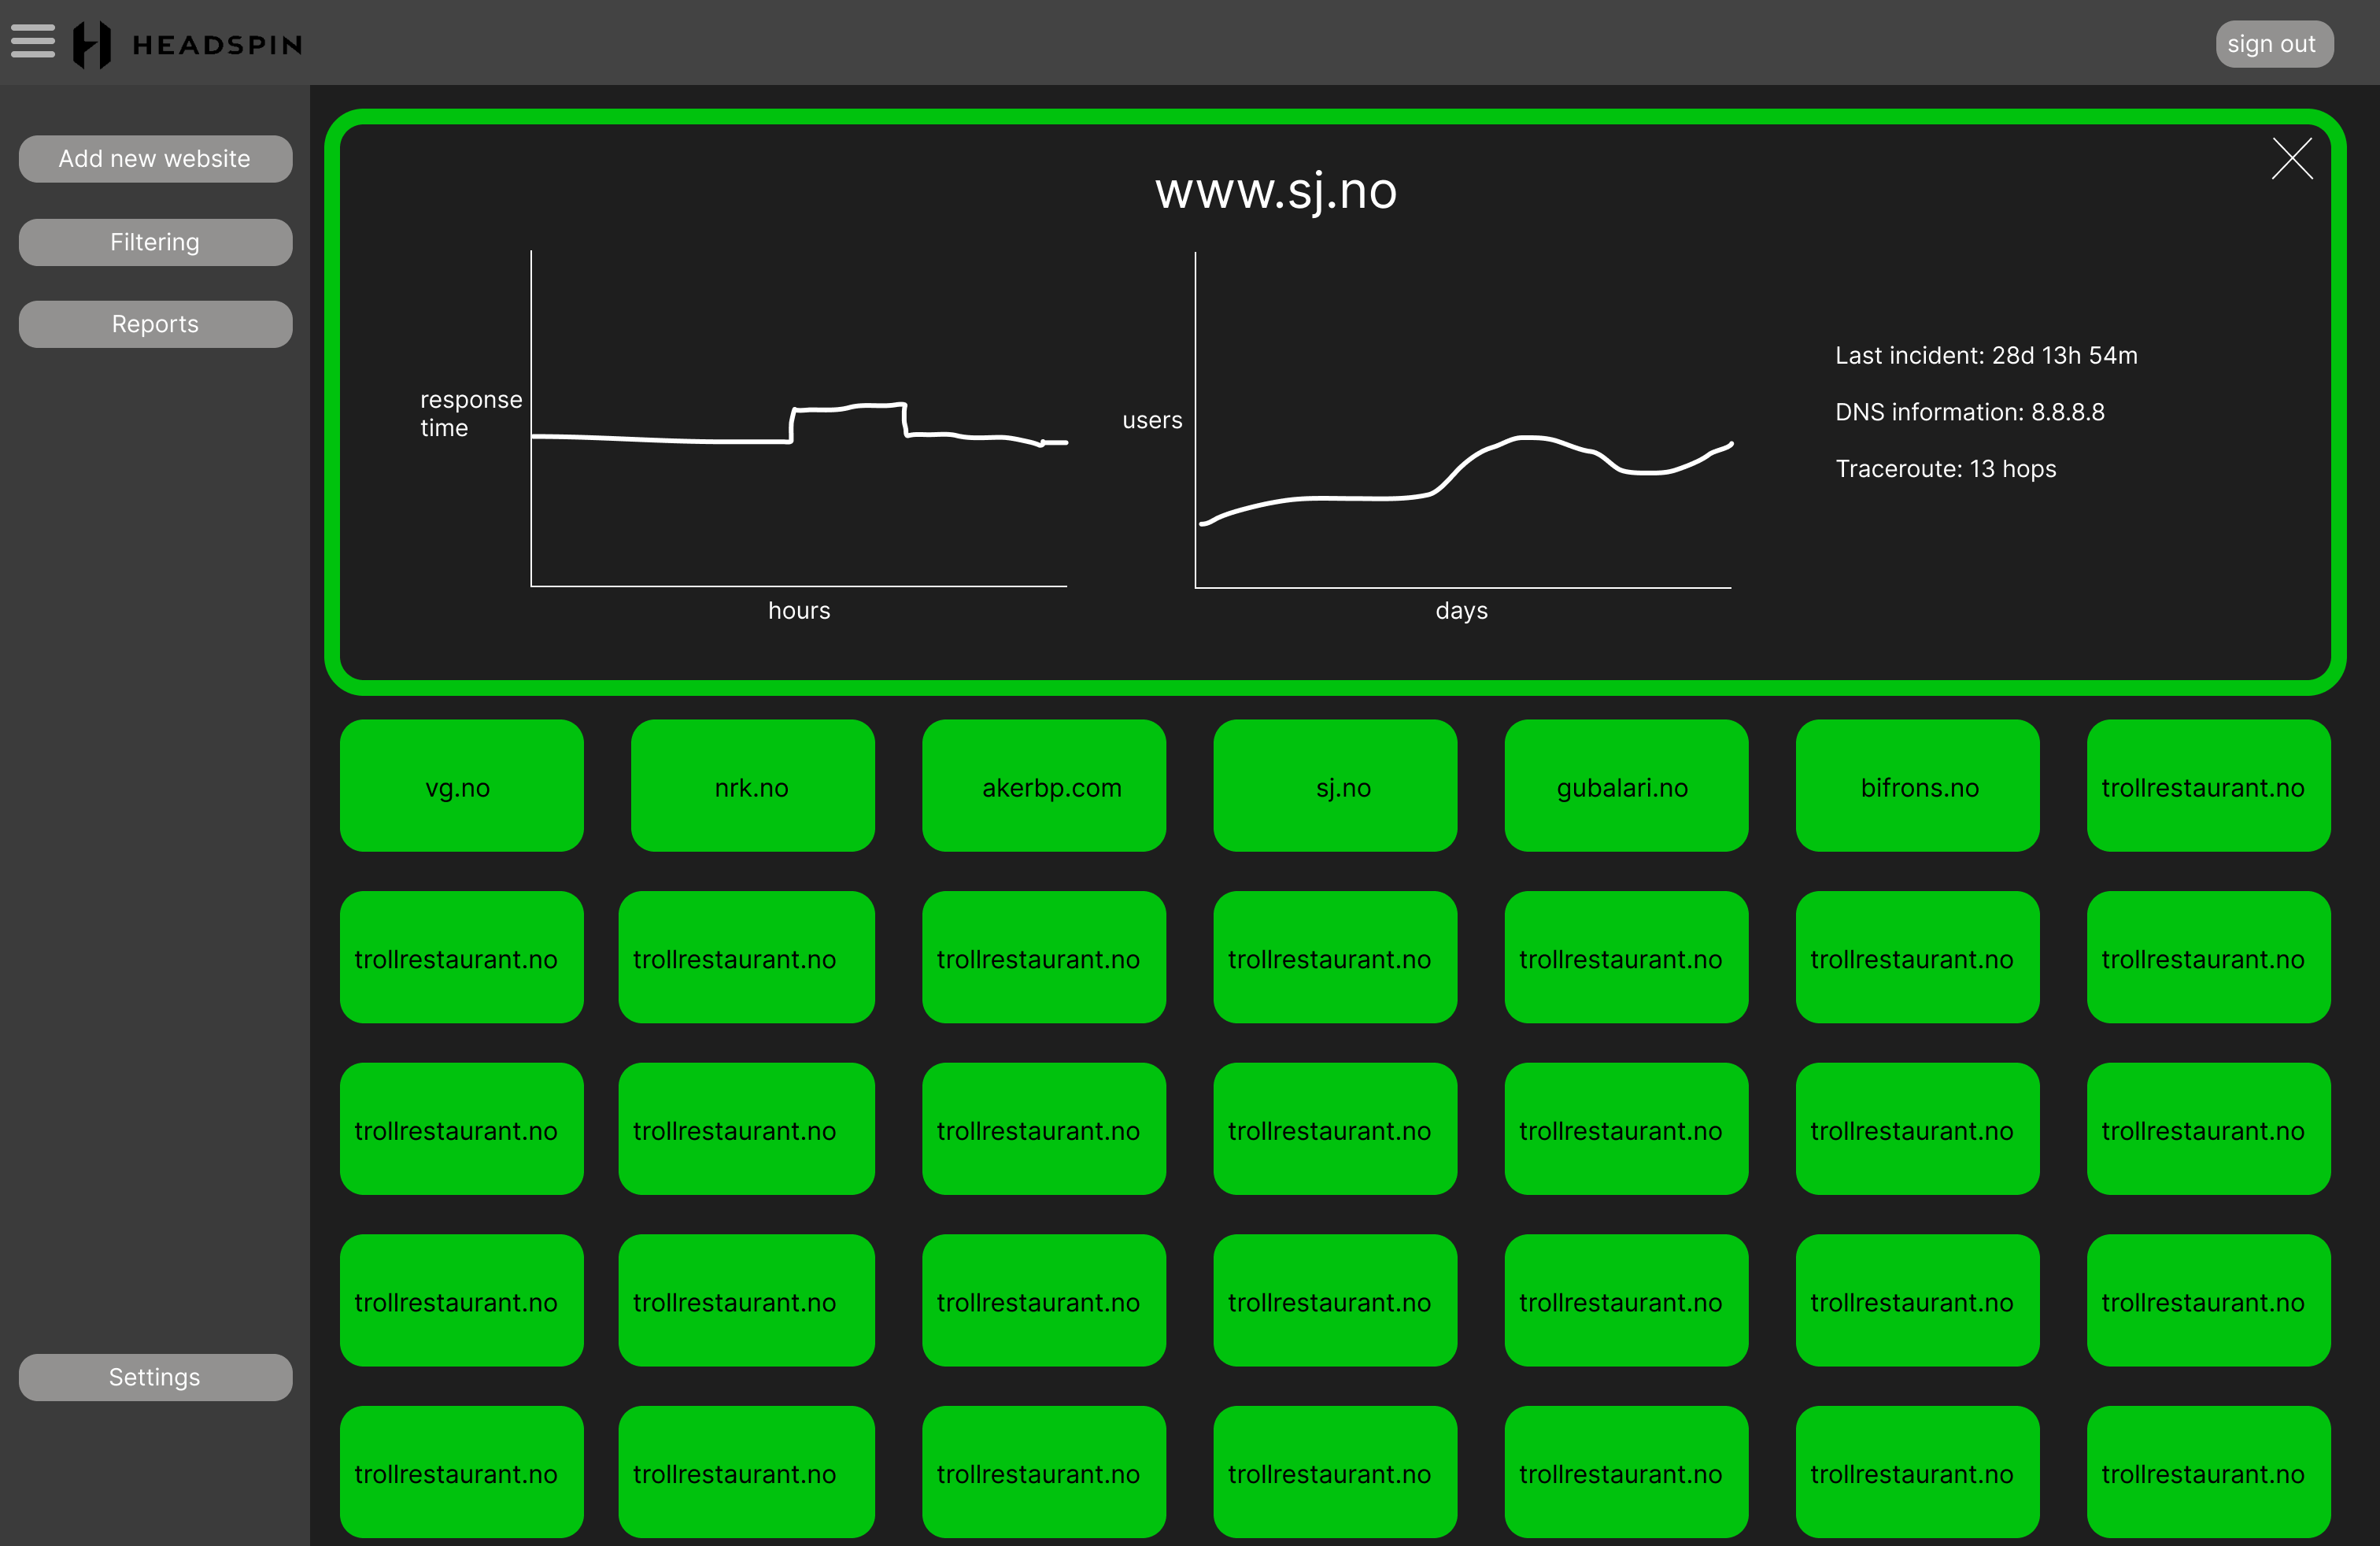
\includegraphics[width=1\linewidth]{figures/prototype_dashboard.png}
    \caption{Prototype of monitoring dashboard}
    \label{o_dash}
\end{figure}



\subsection{Refined Requirements for Development}
\label{subsec:reqs_after_proto}

The insights gathered from both the stakeholder clarification meeting and \textbf{\hyperref[subsec:user_testing]{user test 1}} were consolidated into a refined set of functional and non-functional requirements.  One important design element that changed after the prototype was that we moved away from completely green or red cards on the dashboard, to instead display status in a more visually appealing way. This is what eventually resulted in the final design for the website cards (see \ref{subsubsec:website_card_design}). The following tables present the requirements used throughout the development phase to guide implementation, prioritize features, and support evaluation.


\begin{table}[H]
    \centering
    \caption{Refined Functional Requirements}
    \label{tab:functional_reqs_refined}
    \begin{tabular}{|c|>{\raggedright\arraybackslash}p{0.75\linewidth}|c|}
        \hline
        \textbf{Req ID} & \textbf{Requirement Title} & \textbf{Priority} \\
        \hline
        F.1 & Add, edit, and delete monitored websites via the GUI. & High \\
        \hline
        F.2 & Perform automated checks for up/down status. & High \\
        \hline
        F.3 & Display HTTP status, response time, and uptime history. & High \\
        \hline
        F.4 & Highlight down websites prominently. & High \\
        \hline
        F.5 & Implement user authentication with personalized dashboards. & Medium \\
        \hline
        F.6 & Send alerts via email or SMS. & Medium \\
        \hline
        F.7 & Provide filtering, sorting, and search options. & Medium \\
        \hline
        F.8 & Allow users to define alert thresholds. & Medium \\
        \hline
        F.9 & Let users change check intervals per site. & Medium \\
        \hline
        F.10 & Configure alert destination per website (e.g., email). & Low \\
        \hline
    \end{tabular}
\end{table}

\begin{table}[H]
    \centering
    \caption{Refined Non-Functional Requirements}
    \label{tab:nonfunctional_reqs_refined}
    \begin{tabular}{|c|>{\raggedright\arraybackslash}p{0.75\linewidth}|c|}
        \hline
        \textbf{Req ID} & \textbf{Requirement Title} & \textbf{Priority} \\
        \hline
        NF.1 & Dashboard data must be fresh and updated in near real-time. & High \\
        \hline
        NF.2 & Interface must highlight changes in website status clearly. & High \\
        \hline
        NF.3 & Support monitoring of at least 50 websites without lag. & Medium \\
        \hline
        NF.4 & Ensure maintainability and clear documentation. & Medium \\
        \hline
        NF.5 & Interface should be responsive across screen sizes. & Low \\
        \hline
    \end{tabular}
\end{table}

These refined requirements provided a reference point throughout development and testing. They reflect both stakeholder needs and user-centered refinements gathered from direct testing.

\subsection{Requirement Prioritization Process}
\label{subsec:req_prio_process}

To structure development efficiently, requirements were prioritized based on their impact on usability and project feasibility. High-priority features such as monitoring (F.1–F.4) and real-time updates (NF.1) were implemented first to provide core functionality early. Medium-priority features, including user authentication (F.5) and alert customization (F.8), were added in later iterations. Low-priority requirements, such as per-website email customization (F.10) and varied screen-size responsiveness (NF.5), were addressed as time allowed.


\section{Project Planning}
In this section, different aspects of planning the development process are explored.

\subsection{Timeline and Milestones}
\label{subsec:timeline_and_milestones}

The development process was structured around clearly defined phases and tracked using a Gantt chart (see Figure~\ref{sfig:gantt_dev}). This plan helped guide progress and ensure time was allocated to all major aspects of the project, from planning and development to testing and documentation.

The project began in week 3 with a six-week phase for requirement elicitation, which included reviewing the assignment brief and conducting meetings with stakeholders. In parallel, relevant theory was reviewed from week 5 to week 12 to inform design and development decisions, especially those tied to usability and system architecture, to ensure we could answer \hyperref[subsec:RQ2]{Research Question. 2}.

Prototype development started in week 9 and lasted for two weeks, followed closely by the first round of user testing in weeks 10–11. Feedback from this testing helped refine the system’s design and update requirements.

Product development took place primarily between weeks 8 and 15, during which the main system features were implemented iteratively. This period also included work on authentication, monitoring logic, the alert system, and frontend components. Product evaluation and improvement were prioritized from weeks 15 to 18, guided by new test results and stakeholder feedback (see \ref{subsubsec:compiled_results_mvp}.

Finally, documentation spanned from week 8 to week 19, running in parallel with development and testing to ensure project records, diagrams, and user-facing explanations were consistently updated.

\begin{figure}[H]
    \centering
    \makebox[\textwidth][c]{\includegraphics[width=1.2\textwidth]{figures/gantt_dev.png}}
    \caption{Gantt chart - Development}
    \label{sfig:gantt_dev}
\end{figure}

\subsection{Risk Analysis and Mitigation}

Risk management is a critical component of project planning. We conducted a risk assessment to identify potential challenges and determine appropriate mitigation strategies.

Risks were analyzed based on two factors. The likelihood that a risk occurs, and the severity of it's consequences.  The most relevant risks for our project are summarized below:

\begin{itemize}

    \item \textbf{R1: Time constraints} - With a tight delivery deadline, delays in one phase quickly affect other phases, and the project as a whole.
    \item \textbf{R2: Lack of technical experience or knowledge} - Could delay development or introduce architectural mistakes.
    \item \textbf{R3: Data loss} - Loss of project code or documentation could set us back.
    \item \textbf{R4: Team member absence}
    \item \textbf{R5: Changing requirements}
    \item \end{itemize}

These risks were positioned on a standard risk matrix adapted from Sutton (2021), which categorizes risk severity based on likelihood and impact (see Figure~\ref{fig:risk_matrix}). Higher values (e.g., 21–25) represent more critical risks.

\begin{figure}[H]
    \centering
    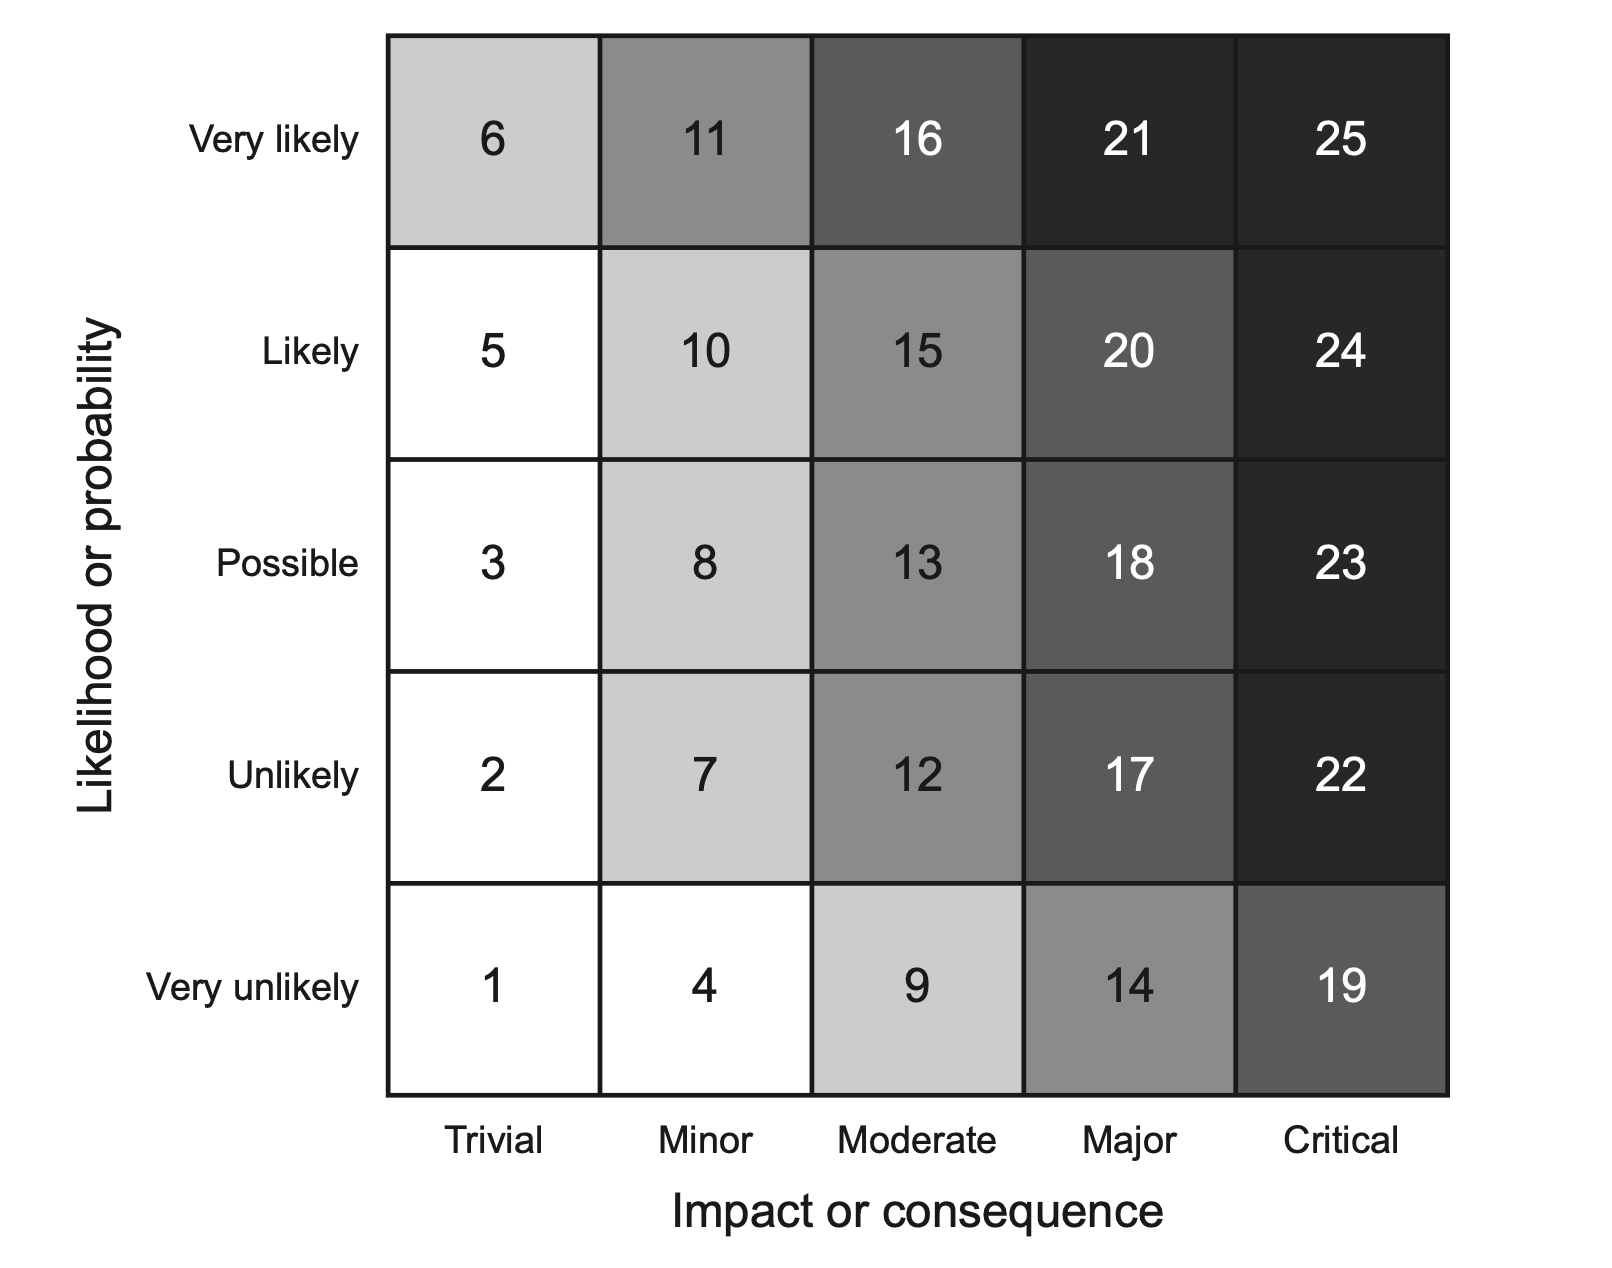
\includegraphics[width=0.8\linewidth]{figures/risk_matrix.png}
    \caption{Risk Matrix \autocite[Figure 6.2]{Sutton2021}}
    \label{fig:risk_matrix}
\end{figure}

Based on this assessment, R1 (Time constraints) and R2 (Requirement ambiguity) were identified as the most severe and likely to occur. Several steps were taken to mitigate these risks:

\begin{itemize}
    \item A detailed project timeline with clear milestones was established, supported by a Kanban-based workflow.
    \item Stakeholder communication was maintained throughout the project to prevent ambiguity and misalignment.
    \item Prototyping and early user testing helped clarify unclear requirements before full implementation.
    \item Features were prioritized based on impact and complexity to maintain focus on core functionality.
    \item Automated testing (via Cypress) was introduced to improve coverage and reduce reliance on manual verification.
\end{itemize}

This structured approach to risk analysis enabled the team to proactively address potential issues, supporting a smoother and more predictable development process.



\section{Technology Stack}
The selection of technologies to use in our application, are guided by our goal of creating a modern, user friendly dashboard application. Each layer of the system, from database and backend to user interface, was built with widely used and standardized technologies.

Figure~\ref{fig:tech_stack}  provides a simplified overview of the stack architecture. It illustrates the three main layers of the system: the frontend (client-facing interface), the backend (application logic and API handling), and the database (persistent data storage). The arrows indicate the flow of data between these components, with REST API calls connecting the frontend to the backend, and Prisma ORM queries facilitating interaction between the backend and the database.


% stack figure
\begin{figure}[H]
    \centering
    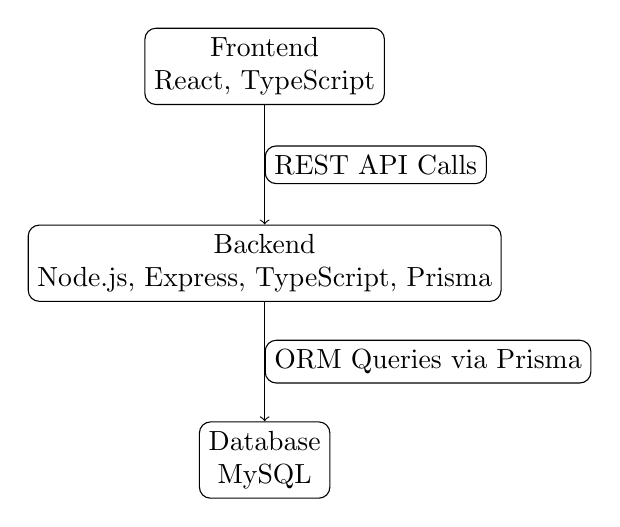
\begin{tikzpicture}[node distance=2.5cm, every node/.style={draw, align=center, rounded corners}]
        \node (frontend) {Frontend \\ React, TypeScript};
        \node (backend) [below of=frontend] {Backend \\ Node.js, Express, TypeScript, Prisma};
        \node (database) [below of=backend] {Database \\ MySQL};

        \draw[->] (frontend) -- node[right] {REST API Calls} (backend);
        \draw[->] (backend) -- node[right] {ORM Queries via Prisma} (database);
    \end{tikzpicture}
    \caption{Simplified Technology Stack Architecture.}
    \label{fig:tech_stack}
\end{figure}


\subsection{Frontend}
Lite innledning til hva som menes mec frontend osv.


\subsubsection{React}
React was chosen for its component-based architecture, which enabled the creation of modular and reusable user interface elements. In our project, the entire dashboard view was built using React components such as \texttt{Navbar}, \texttt{WebsiteCard}, and \texttt{IncidentList}. React’s virtual DOM and efficient rendering allowed for seamless updates to site monitoring data, ensuring that real-time changes could be reflected with minimal performance overhead.

\subsubsection{\gls{vite}}
\gls{vite} is a widely used build tool for React aims to provide faster and leaner development experience for modern web projects.\autocite{viteGuide} Vite's Hot Module Replacement (HMR) which provides near instant updates when code is changed without having to refresh the page, proved very useful during development.

\subsubsection{\gls{typescript}}
\gls{typescript} was used to add static typing to JavaScript. Typescript helped improve code quality


\subsubsection{\gls{mui}}
The project used \gls{mui} as the component library for building the interface. Prebuilt components such as buttons, text fields, and layout grids were used to construct forms and views. The library’s support for responsive design was used to adapt the dashboard to different screen sizes. MUI also helped maintain consistent colors in the user interface.

\subsubsection{Axios}
Axios was used to perform requests from the frontend to the backend API, and for the backend to send data to the fronted. It was chosen for its simplicity, built-in support for promises, and ability to intercept requests and responses. The team also had previous with Axios. Axios allowed us to. The monitoring system also used Axios to check availability of websites. See \autoref{subsubsec:monitoring_logic} for details.


\subsubsection{Chart.js}
Chart.js was used to display data in a visual format. It was integrated into the \texttt{WebsiteCard} component and the \texttt{WebsiteDetails} page to show historical uptime and response time as line charts. Chart.js allowed us to highlight anomalies such as downtime periods by customizing colors and tooltips. The flexibility of this library enabled us to visually communicate performance trends without implementing custom drawing logic.


\subsection{Backend}
The backend of the application was responsible for handling core business logic, database access, scheduled operations, and serving the REST API endpoints consumed by the frontend.

\subsubsection{Node.js}
Node.js was selected as the runtime environment for the backend server. Node is widely adopted adoption, and has a large ecosystem and is well documented. The team also has previous experience working with Node-apps. 

\subsubsection{Prisma ORM}
Prisma was used as the Object-Relational Mapping (\textbf{\acrshort{orm}}) tool for interacting with the database. A schema was defined to model users, monitored websites, and associated alert settings. Prisma’s type-safe query methods were used in backend routes to read and write data. This reduced the need for raw  queries and allowed data models to remain in sync with the database schema throughout development. Prisma also allows for switching between database solutions with minimal effort.

\subsubsection{Scheduled jobs with \gls{cron}}
We use \textbf{cron} to schedule checks for websites based on user defined intervals. We also regularly monitored for status changes to website based the conducted checks,  as well as running regular cleanup of the database.

\subsection{Database}
We needed a database that allowed storing large quantities of data, as each check of a monitored website would be stored in the database for some time.

\subsubsection{MySQL}
We chose to use a MySQL database system as that is what the team has worked with before. See \autoref{fig:mysql_schema} for our database model.



\begin{figure}[H]
    \centering
    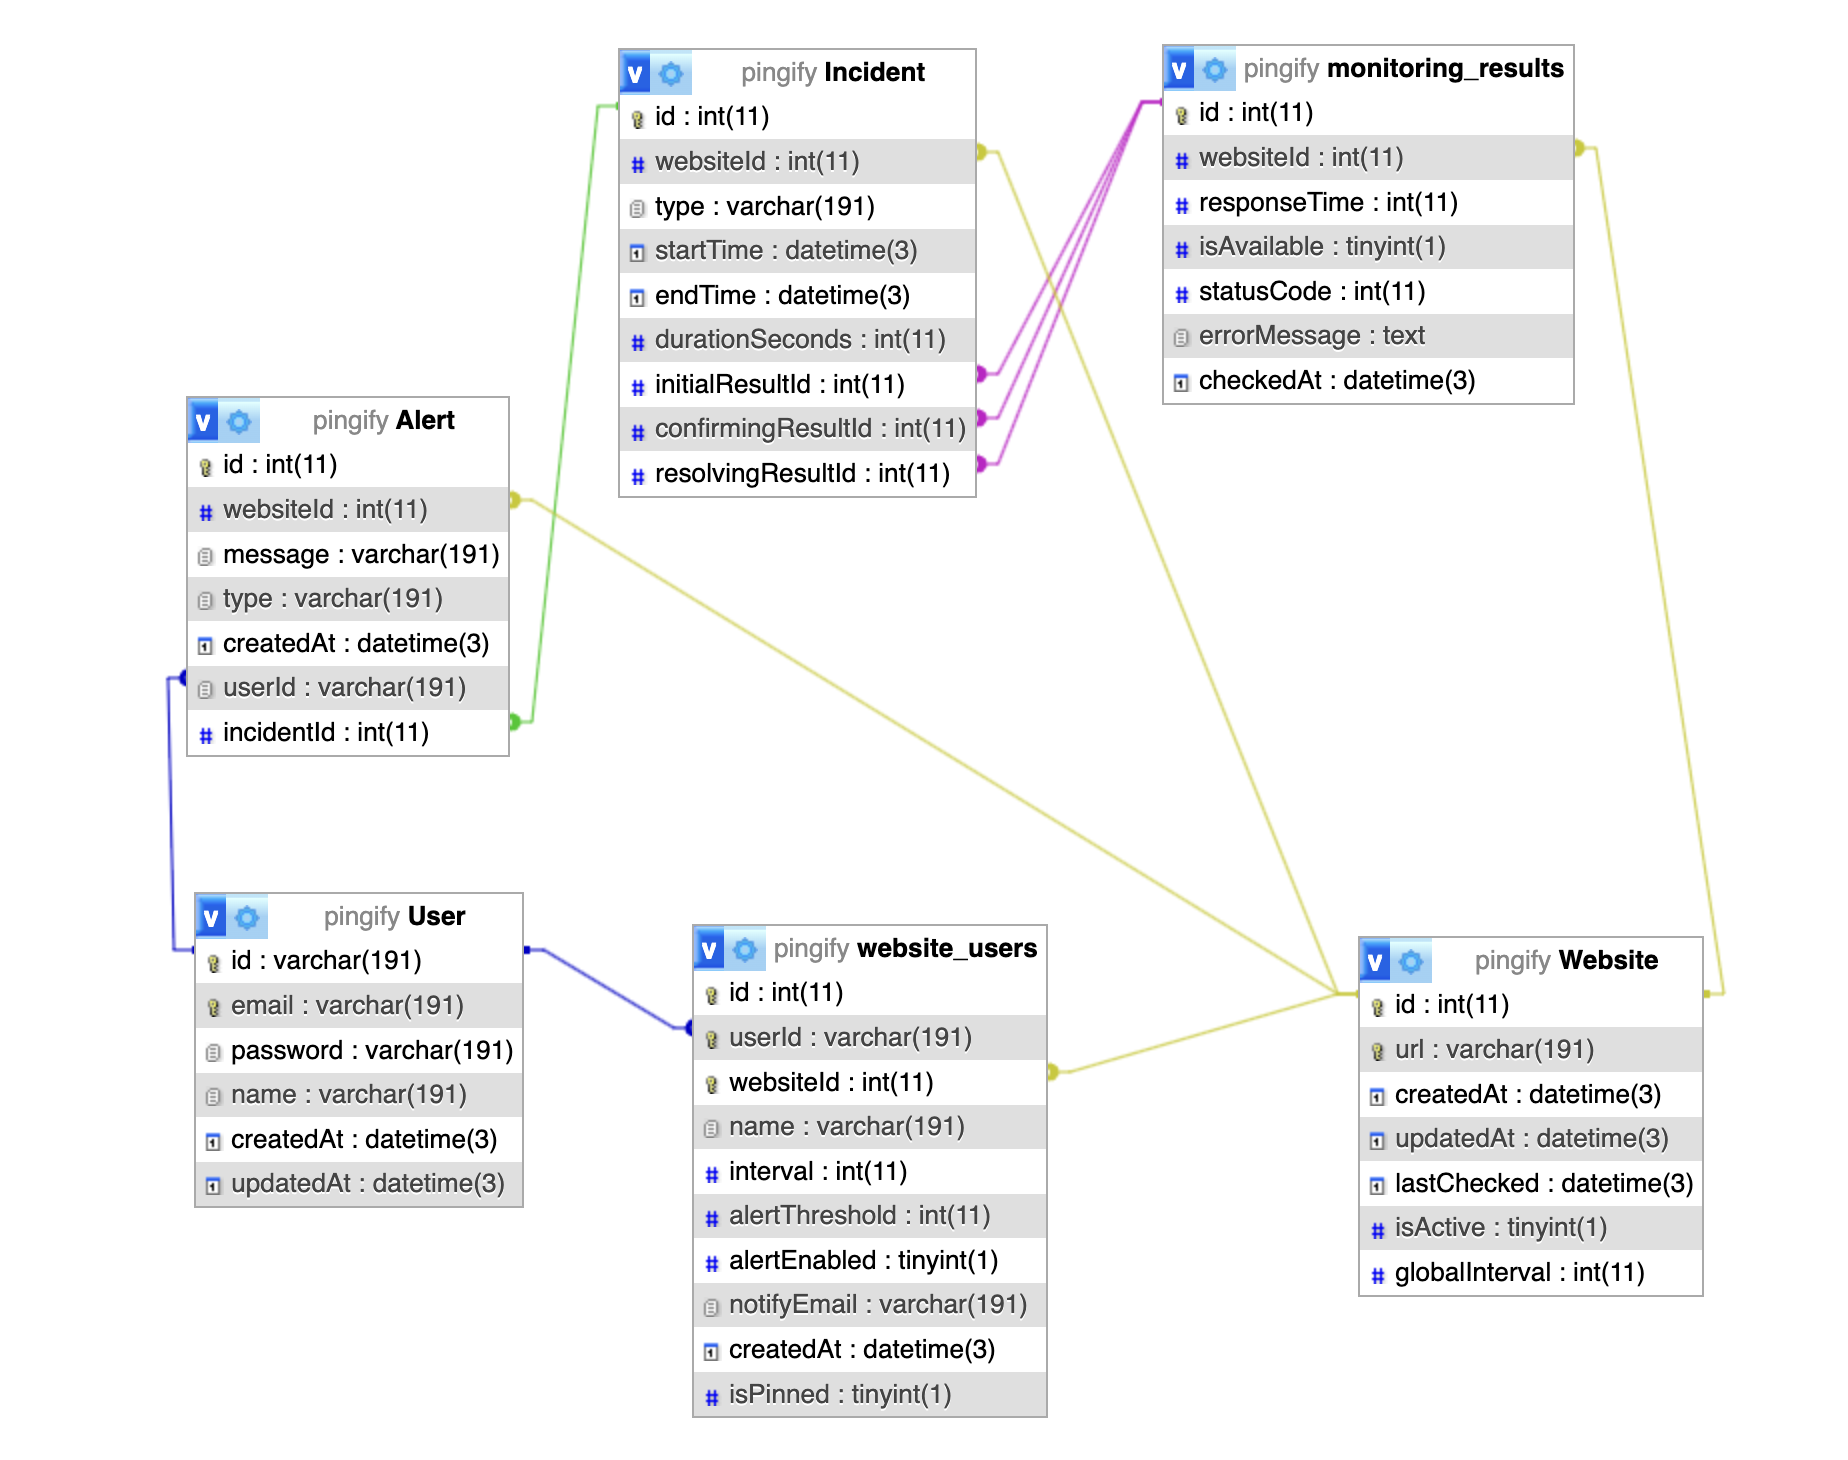
\includegraphics[width=1\textwidth]{figures/mysql_scheme.png}
    \caption{Database schema as implemented in MySQL.}
    \label{fig:mysql_schema}
\end{figure}


\subsection{Collaboration Tools}
This section intends to describe how we actively progressed our development process with the help of these tools.

\subsubsection{\gls{github}}
\gls{github} was used as a tool to maintain the codebase and facilitate collaborative development. By using Git branches, we were able to work on different components of the system in parallel without interfering with work of other team members. Each new feature or bugfix was developed in a separate branch, and changes were merged into the main branch through pull requests. This workflow allowed for code review, discussion, and quality control before integration. We also used Github Pipeline during testing and deployment, which is explanined further in  section \ref{sec:testing_deployment}.

\subsubsection{Jira Software} 
\label{subsubsec:jira}

To implement Kanban, we used Jira Software. Jira is a project management tool that supports agile workflows \cite{Jira}. Jira's issue board and backlog features allowed us to create and manage tasks throughout development. Issues were derived from application requirements and broken down into smaller tasks. A new Git branch was created when an issue moved to "WORKING ON", and upon completion and successful merging, it was moved to "COMPLETED".

We used Jira’s assign feature to track ownership. Team members could choose issues based on preference, promoting flexibility and smoother collaboration.

We used a four-column board: "TODO", "WORKING ON", "COMPLETED", and "BUGS", as shown in Figure~\ref{fig:kanban_board}. Column limits were set to avoid overload and maintain a steady workflow.

\begin{figure}[H] 
\centering 
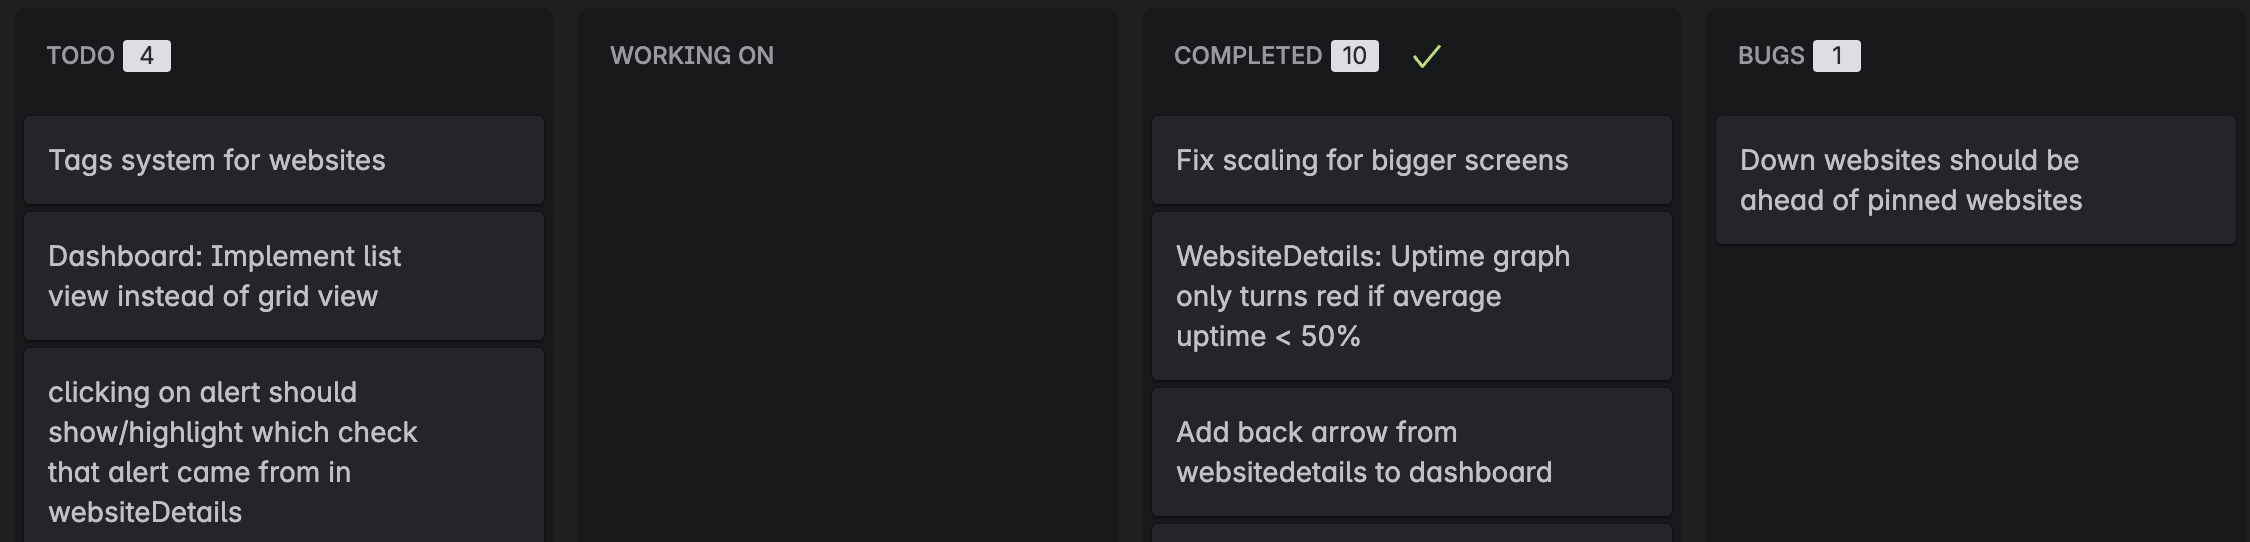
\includegraphics[width=1\linewidth]{figures/kanbanboard.png} 
\caption{Kanban Board} 
\label{fig:kanban_board} 
\end{figure}


\subsubsection{AI Tools}
We used AI tools like ChatGPT, as problem solving tools when encountering errors while coding.
AI tools also generally helped improve efficiency throughout the development process, by suggesting improvements and generating code to tackle difficult problems.

\section{Testing and Deployment}
\label{sec:testing_deployment}
We employed a structured approach to testing and deployment to ensure software quality and maintainability. This included end-to-end testing, automated CI workflows, and systematic bug tracking.


\subsection{End to End Testing}

As we developed a \gls{fullstack} application, we figured it made the most sense to perform \gls{e2e-testing}, to test as much of the application as possible in the most efficient and least time costly way possible. We used \gls{cypress} as it is widely used, well documented, and because we have prior experience working with it. Our Cypress tests involved logging in, clicking on a website card on the dashboard, and verifying that the resulting page renders, as seen in figure \ref{fig:cypress_test}.



\begin{figure}[H]
    \centering
    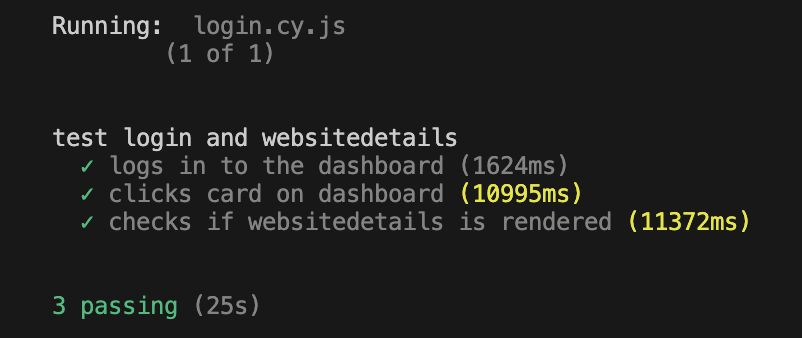
\includegraphics[width=0.5\linewidth]{figures/cypress_test.png}
    \caption{Cypress end-to-end test result}
    \label{fig:cypress_test}
\end{figure}

\subsection{GitHub Actions}

To maintain code quality and ensure continuous integration throughout development, we utilized \textbf{\gls{github-actions}} to automate our testing pipeline. Specifically, we configured GitHub Actions to run on every pull request targeting the main branch. This setup helped us catch issues early and enforce consistent standards across the codebase.

Our workflow was divided into two separate \textbf{\gls{yaml}} configuration files:
\begin{itemize}
    \item One workflow was dedicated to running our Cypress end-to-end tests.
    \item The other handled prettier, linting and static type checking using TypeScript as seen in \ref{fig:lint_typecheck_ci}.
\end{itemize}

Although both workflows were triggered by the same event ruleset, they were deliberately split for easier maintenance, debugging, and clearer feedback in the GitHub interface.

\begin{figure}[H]
    \centering
    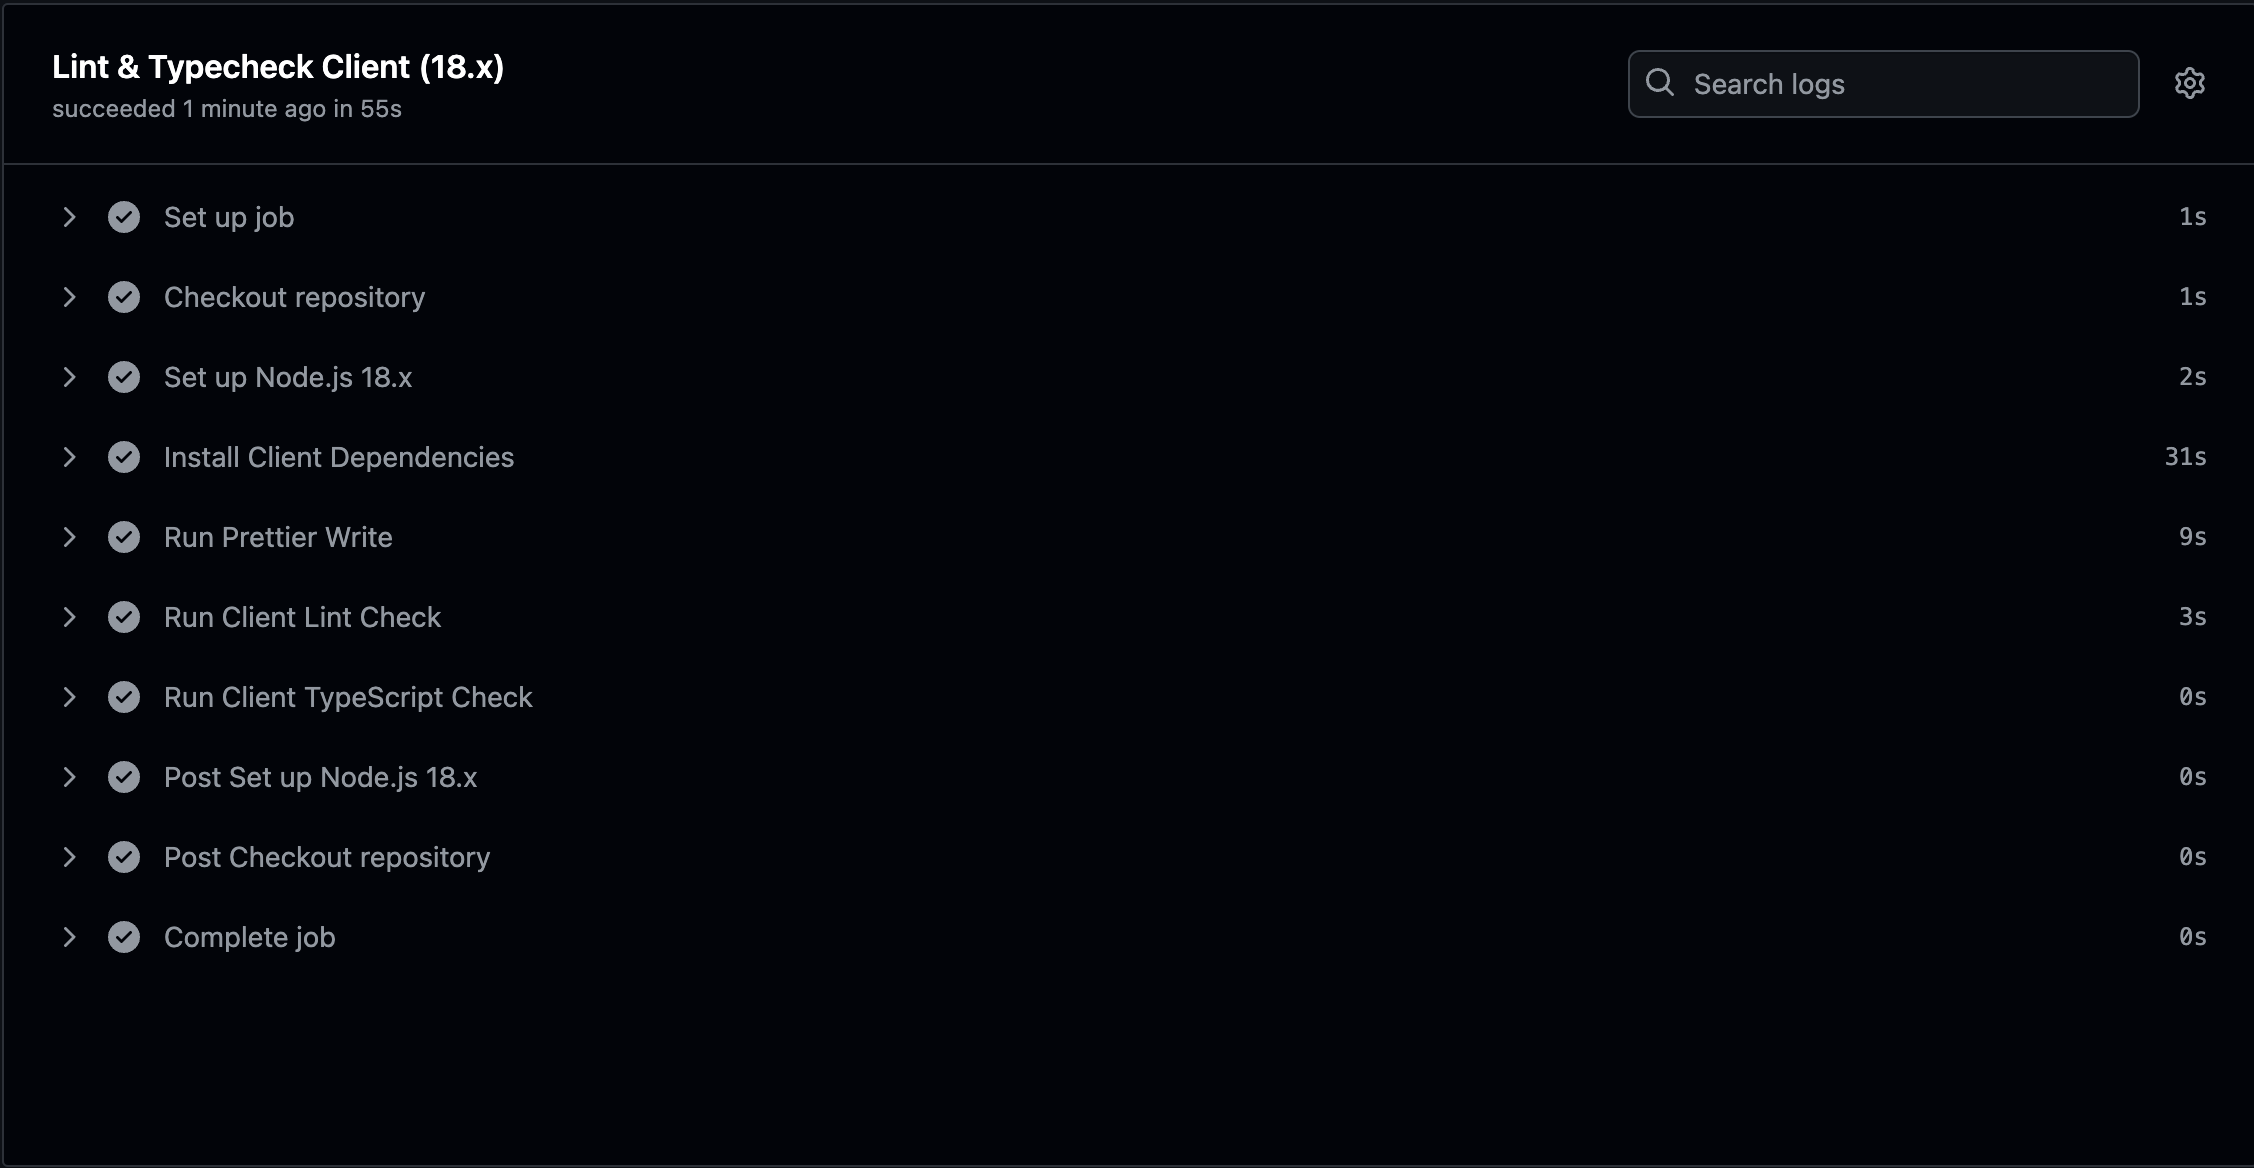
\includegraphics[width=1\linewidth]{figures/lint_typecheck_ci.png}
    \caption{CI pipeline running prettier, linting and type checking via GitHub Actions}
    \label{fig:lint_typecheck_ci}
\end{figure}



\subsection{Bug Tracking and Fixing}
To efficiently track bugs, we used a separate column in our Kanban-board to track known bugs. Throughout development we aimed to fix bugs as they were discovered.
Most bugs were visual errors, which were easily fixed. But some were caught only when actively testing our product and looking for them.
%bruke bilder her for å vise eksempel på bug?


\section{Application Status: End of Development Process}
\label{sec:status_at_completion}
tekst om hele prosessen som kommer under

\subsection{System Design}
The figure below shows all the different pages and options the user has, to give an overview of the application before discussing logic and moving on to component specifics and design choices.

%figur av hele siden oppsumert
\begin{figure}[htbp]
        \centering
        \includegraphics[width=\textwidth]{figures/Sitemap.png}
        \caption{Sitemap}
        \label{sfig:sitemap}
\end{figure} 

\subsubsection{Monitoring Logic}
\label{subsubsec:monitoring_logic}
The monitoring system was implemented using \gls{axios} and \gls{cron}. Each monitored website was checked at a user-defined interval, with scheduled jobs executing \acrshort{http} requests to collect two key metrics: the \acrshort{http} status code and the response time to the first byte. These values were stored in the database for further processing.

Collected data was used to generate uptime statistics and response time charts within the user interface. The monitoring logic relied exclusively on the \acrshort{http} status code and timing information provided by \gls{axios} to determine whether a website was considered up or down.

If a timeout occurred during a check, the result was marked as failed (red) in the system. A follow-up check was automatically scheduled 60 seconds later to verify whether the issue persisted. If the second check also failed, an incident is created, and an alert with subsequent email notification was sent if the user had alerts enabled for that website.

In addition to downtime alerts, users could define custom thresholds for acceptable response times. If a site exceeded this threshold, a "slow" alert was created. These thresholds were configurable per website, allowing users to adjust expectations for sites that consistently load more slowly.

\subsubsection{Alert System}

The alert system was integrated into the scheduled monitoring jobs. When regular monitoring check for any given website failed, the backend evaluated whether the failure met the criteria for triggering an alert. These criteria included threshold conditions defined by the user, such as consecutive failures or prolonged downtime.

Once the conditions were met, an alert record was created in the database. 
The backend server the  sends an email to a user specified email-address for that website, if the user has alerts configured. To prevent sending unnecessary alerts, the system only allowed for one active alert per website for each user. The user had to manually delete an alert to receive a new one.

% stemmer for å fjerne dette nå, flyttet incident teori ned til dashboard

The alert system is designed in a way not to only notify users of issues, but also to do so in a manner that supports usability, clarity, and minimizes cognitive load. Achieving this is done by designing the system in line with Stephen Few's principles of simplicity and critical value exceptions ( see \autoref{subsubsec:principle_simplicity}. Rather than overwhelming the user with every failure, the system uses threshold conditions, both user-defined and system standard. This approach ensures that only meaningful anomalies surface, aligning with Few's suggestions that dashboards should highlight actionable information without excessive clutter. The alert logic reinforces Don Norman's principle of constraints by preventing redundant alerts, guiding user attention, and reducing unnecessary interruptions (see \autoref{par:constraints}. 

\subsubsection{Incidents System}
After \hyperref[subsec:user_testing]{user test 2}, which focused on application flow, the team received feedback explaining that test subjects wanted a better way to identify why a red/orange status indicator was displayed. This led to a new functional requirement F.11 being written, to develop an incident system.

The incident system works by adding an incident to the database if a monitored website has been down or slow for two consecutive checks. This moves the dashboard card  for that website to the top of the Dashboard, as well as displaying a yellow/red status indicator depending on the severity of the incident (down/slow). Past and present incidents can be displayed in a list on a separate page, or for a specific website by clicking on corresponding card on the dashboard.

\subsubsection{User Authentication}
As described in \autoref{sec:def_req}, user authentication was not originally a requirement for the application. However, after feedback gathered during the requirement elicitation process, it was deemed beneficial that users could have their own dashboard with custom websites, instead of one central dashboard that everyone had access to. Based on this, a robust authentication system using \textbf{\gls{jsonwebtoken}} was implemented. This enabled user registration and login/logout functionality, as well as each user only having access to their own personal dashboard.



\subsection{Implementation}
This section describes the most important React components used in the frontend, focusing on their responsibilities, interactions, and design considerations.

The implementation draws on design theory to address usability in the dashboard interface. Principles from Stephen Few (see \ref{subsec:principles_of_dashboard_design}), Don Norman (see \ref{subsubsec:don_norman_design_principles}), and Jakob Nielsen (see \ref{subsubsec:connecting_visual_and_interaction_design}) influenced decisions related to layout, interaction design, and visual communication.


\subsection{Implementation}
This section outlines the core React components used in the frontend, focusing on their responsibilities, interactions, and design rationale.

The implementation draws directly on the design theories discussed in Chapter~\ref{ch:theory}. Layout and data prioritization were guided by Few’s dashboard principles (\autoref{subsec:principles_of_dashboard_design}), emphasizing clarity, simplicity, and the visibility of critical information. Interaction patterns follow Norman’s principles of affordance, feedback, and visibility (\autoref{subsubsec:don_norman_design_principles}), shaping how users engage with the system. Nielsen’s heuristics (\autoref{subsubsec:connecting_visual_and_interaction_design}) informed the use of consistency, status indicators, and error handling.

Together, these frameworks supported the development of a frontend that is both functional and user-friendly, grounded in established design theory.



\subsubsection{Dashboard Page}
The dashboard page serves as the main interface of the application. It displays near real-time data on website availability and uptime statistics, acting as the central point of user interaction (see \ref{sec:website_monitoring}). In line with Stephen Few's definition, the dashboard is designed to present the most important information in a clear and concise way on a single screen, so the user can monitor important information at a glance, as stated in \ref{subsec:what_is_dashboard}. 

\paragraph{Dashboard Behavior}

The dashboard is the first screen users see after logging in and is where they are expected to spend most of their time. It supports operational monitoring by immediately highlighting when something requires attention. This aligns with Few's concept of critical value exceptions (see \ref{subsubsec:principle_simplicity}), clearly showcasing when user action is needed, and is supported by Nielsen's principle of visibility of system status, which says the system should always keep users informed about what's going on (see \ref{par:visibility_system_status}). 

\paragraph{Dashboard Layout and Design}
The layout applies several of the Gestalt principles, which Few integrates in his theory of dashboard design, as outlined in Section \ref{subsubsec:gestalt_principles}, to organize and simplify the presentation of information. The principle of proximity is used for related data, like uptime and number of incidents, being placed close together to show they belong together. The principle of enclosure, where bordered and shaded sections are used to group data, making the page easier to scan. Using the principle of similarity, with consistent use of fonts, icons, and spacing to reinforce visual coherence. This also supports Norman's principle of consistency by helping users form a predictable mental model of the interface (see \ref{subsubsec:don_norman_design_principles}).

The principle of simplicity is a key focus throughout (see \ref{subsubsec:principle_simplicity}) development. We aim to minimize clutter, using summaries and graphs instead of full data tables and only highlighting detailed data when necessary. This helps to reduce cognitive load and allows users to understand the most critical information quickly

Colour theory is applied deliberately throughout the application (see \ref{subsec:colour_theory}). Warm colours like red and orange are used to indicate warnings or issues that need attention, while cool colours like green and blue indicate stability or success. Complementary colour pairs, such as red and green, are used to create strong visual contrast between positive and negative states. This not only enhances visibility but draws the users attention where it's needed the most. These choices follow traditional colour psychology and support Nielsen's visibility of system status heuristic, helping users immediately understand what is functioning correctly and what requires action (see \ref{par:visibility}).

Instead of treating all monitored websites equally on the dashboard, the system elevates cards representing websites with active incidents. Giving these anomalies visual priority, both through repositioning and color indicators, supports Few's critical value exception (see \ref{subsubsec:principle_simplicity}.

From a visual design perspective, the relocation of the Website Card component reinforces the Gestalt principle of proximity by grouping the most critical elements at the top of the interface. This dynamic update of the interface is supported by Nielsen's heuristic of system status visibility. By clearly informing the user that the system has detected an issue and communicating this change in real time, the dashboard improves both usability and situational awareness, allowing users to focus attention where it is most needed (see \ref{par:visibility_system_status}.

In terms of interaction, several of Norman's principles (\ref{subsubsec:don_norman_design_principles}) are actively applied:

\begin{itemize}
    \item \textbf{Feedback:} The interface gives immediate visual responses to user actions, such as highlighting or updating components in real-time. For example, hovering over the graph for response times reveals tooltips with detailed values.
    \item \textbf{Affordance:} Interactive elements, like the filter field, sort menu, and new website card, use visual cues (icons, shadows, hover effects) to indicate their functionality. This makes their purpose intuitive even without explicit instructions.
    \item \textbf{Visibility:} Core system actions and status indicators are placed front and center, such as overall website status, uptime, incident, or change in website status, ensuring that users can immediately interpret the monitoring state without effort.
    \item \textbf{Consistency:} The cards for each website are identically structured, and repeated UI components behave the same across the dashboard. This reduces the learning curve and improves usability.
\end{itemize}

Together, these design and interaction principles ensure that the dashboard is not only visually clean but also intuitive and easy to use.
    

\subsubsection{Website Card Component}
\label{subsubsec:website_card}

\paragraph{Website Card Behavior}

The website card is a core UI component responsible for displaying the real-time status of a single monitored website. It receives props, such as URL, \acrshort{http} status, last response time, and a list of recent checks, all passed from the backend via API calls.

The component conditionally renders its UI based on the received data.
If the \acrshort{http} status indicates downtime, the card communicates this with a red "Offline" label and a critical warning message. If the site is online, the card displays key metrics such as response time and uptime percentage for the last 24 hours. The visual state of the card updates automatically when new monitoring data arrives from the backend server.



\paragraph{Website Card: Layout and Design}
\label{par:website_card_design}

The website card is designed to communicate status clearly and efficiently. Following Stephen Few's dashboard design principles the component presents a compact, information-rich summary of a website's operational state. By avoiding information overload and using visual prioritization, the component allows users to quickly interpret a site's status at a glance, which is essential for an operational dashboard (see, \ref{subsubsec:different_types_dashboards}). 

Related metrics such as response time, uptime percentage, and current status are close together within the card. This supports the Gestalt principle of proximity, helping users visually connect related data points without cognitive effort. 

The visual design of the website card also benefits from consistent styling across all cards. Typography, iconography, and layout are kept uniform, which reinforces predictability and aligns with Nielsen's heuristic of consistency of standards (see \ref{par:consistency_and_standards}). This helps users build a mental model that applies across cards, regardless of which website is being monitored. 

Colour, together with relevant data or icons, is an essential part of how the website card communicates website status. A green badge signal that a website is operational, orange highlights slower response time, and red indicates downtime or failure. These colours are chosen for their intuitive emotional associations and strong contrast, supporting rapid interpretation. 

Together, these visual and behavioral design choices ensure that each website card contributes meaningfully to the overall usability of the dashboard. Supporting quick decision making and continuous system awareness.

\begin{figure}[H]
    \centering
    \begin{subfigure}[b]{0.45\textwidth}
        \centering
        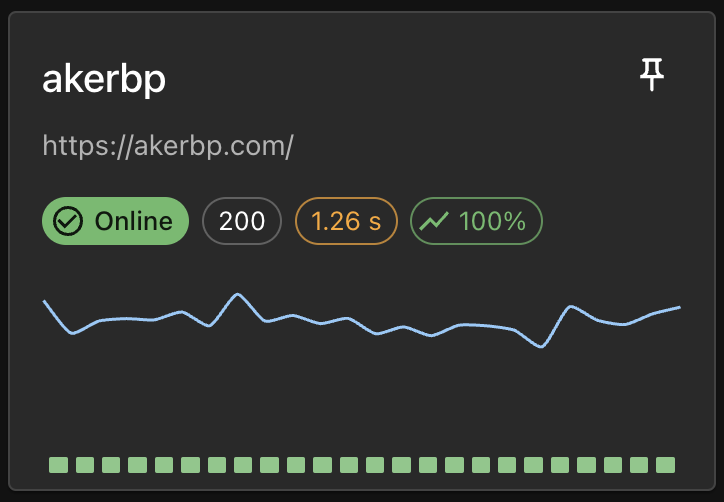
\includegraphics[width=\textwidth]{figures/websiteCard.png}
        \caption{Website Card showing a site currently online}
        \label{fig:websitecard-component}
    \end{subfigure}
    \hfill
    \begin{subfigure}[b]{0.45\textwidth}
        \centering
        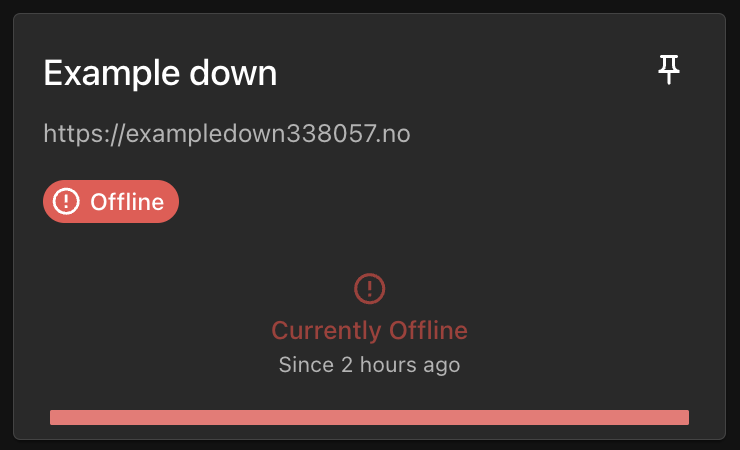
\includegraphics[width=\textwidth]{figures/websitecard_down.png}
        \caption{Website Card showing a site currently offline}
        \label{fig:websitecard-component-down}
    \end{subfigure}
    \caption{Visual comparison of the Website Card component in online and offline states}
    \label{fig:websitecard-comparison}
\end{figure}



\subsubsection{Website Details Page}
The Website Details page is one of the main views of the application. It provides more detailed information for a specific website than what is shown on the main dashboard.

\paragraph{Page Behavior}
Users access this page by clicking on a Website Card component. Once navigated, the page dynamically renders several charts and UI elements to present detailed monitoring data fetched from the database. This interaction is outlined in the sequence diagram below (see \autoref{sfig:sequence_diagram}).

\begin{figure}[htbp]
        \centering
        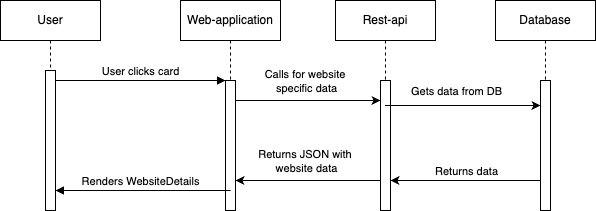
\includegraphics[width=\textwidth]{figures/Sequence_diagram.jpg}
        \caption{Website Details Sequence Diagram}
        \label{sfig:sequence_diagram}
\end{figure}

\paragraph{Website Details: Layout and Design}

According to Stephen Few, a dashboard should make it as easy and seamless as possible to find the information needed to take action (see \ref{subsec:what_is_dashboard}). This idea guided the development of the Website Details page. While the dashboard itself is designed to notify users that action is required, the Website Details page is intended to help users understand what action to take.

To support this, the page displays detailed information about recent incidents, as well as historical data on uptime and response time. These are presented through clear and compact visualizations that makes it easy to interpret patterns and spot anomalies. This follows Few's principles to minimizing cognitive load and making critical information visually accessible at a glance (see \ref{subsubsec:principle_simplicity}.

When an incident is active, a large banner appears at the top of the page, pushing other components down. This draws immediate attention using a combination of icons, descriptive text, and strong color contrasts. 

Interactive elements such as buttons and dropdown filters are designed with Don Norman's principle of affordance in mind (see \ref{par:affordance} Their shape, labeling and visual style suggest their function clearly, helping users understand how to interact with the interface. The layout also reflects Jakob Nielsen's usability heuristics (see \ref{subsubsec:connecting_visual_and_interaction_design}. The system's status is always visible through updated status indicators and live chats, ensuring that users are kept informed. The use of consistent styles, icons, and layout patterns across the application reduces confusion and supports a more user-friendly experience. 


\begin{figure}[H]
    \centering
    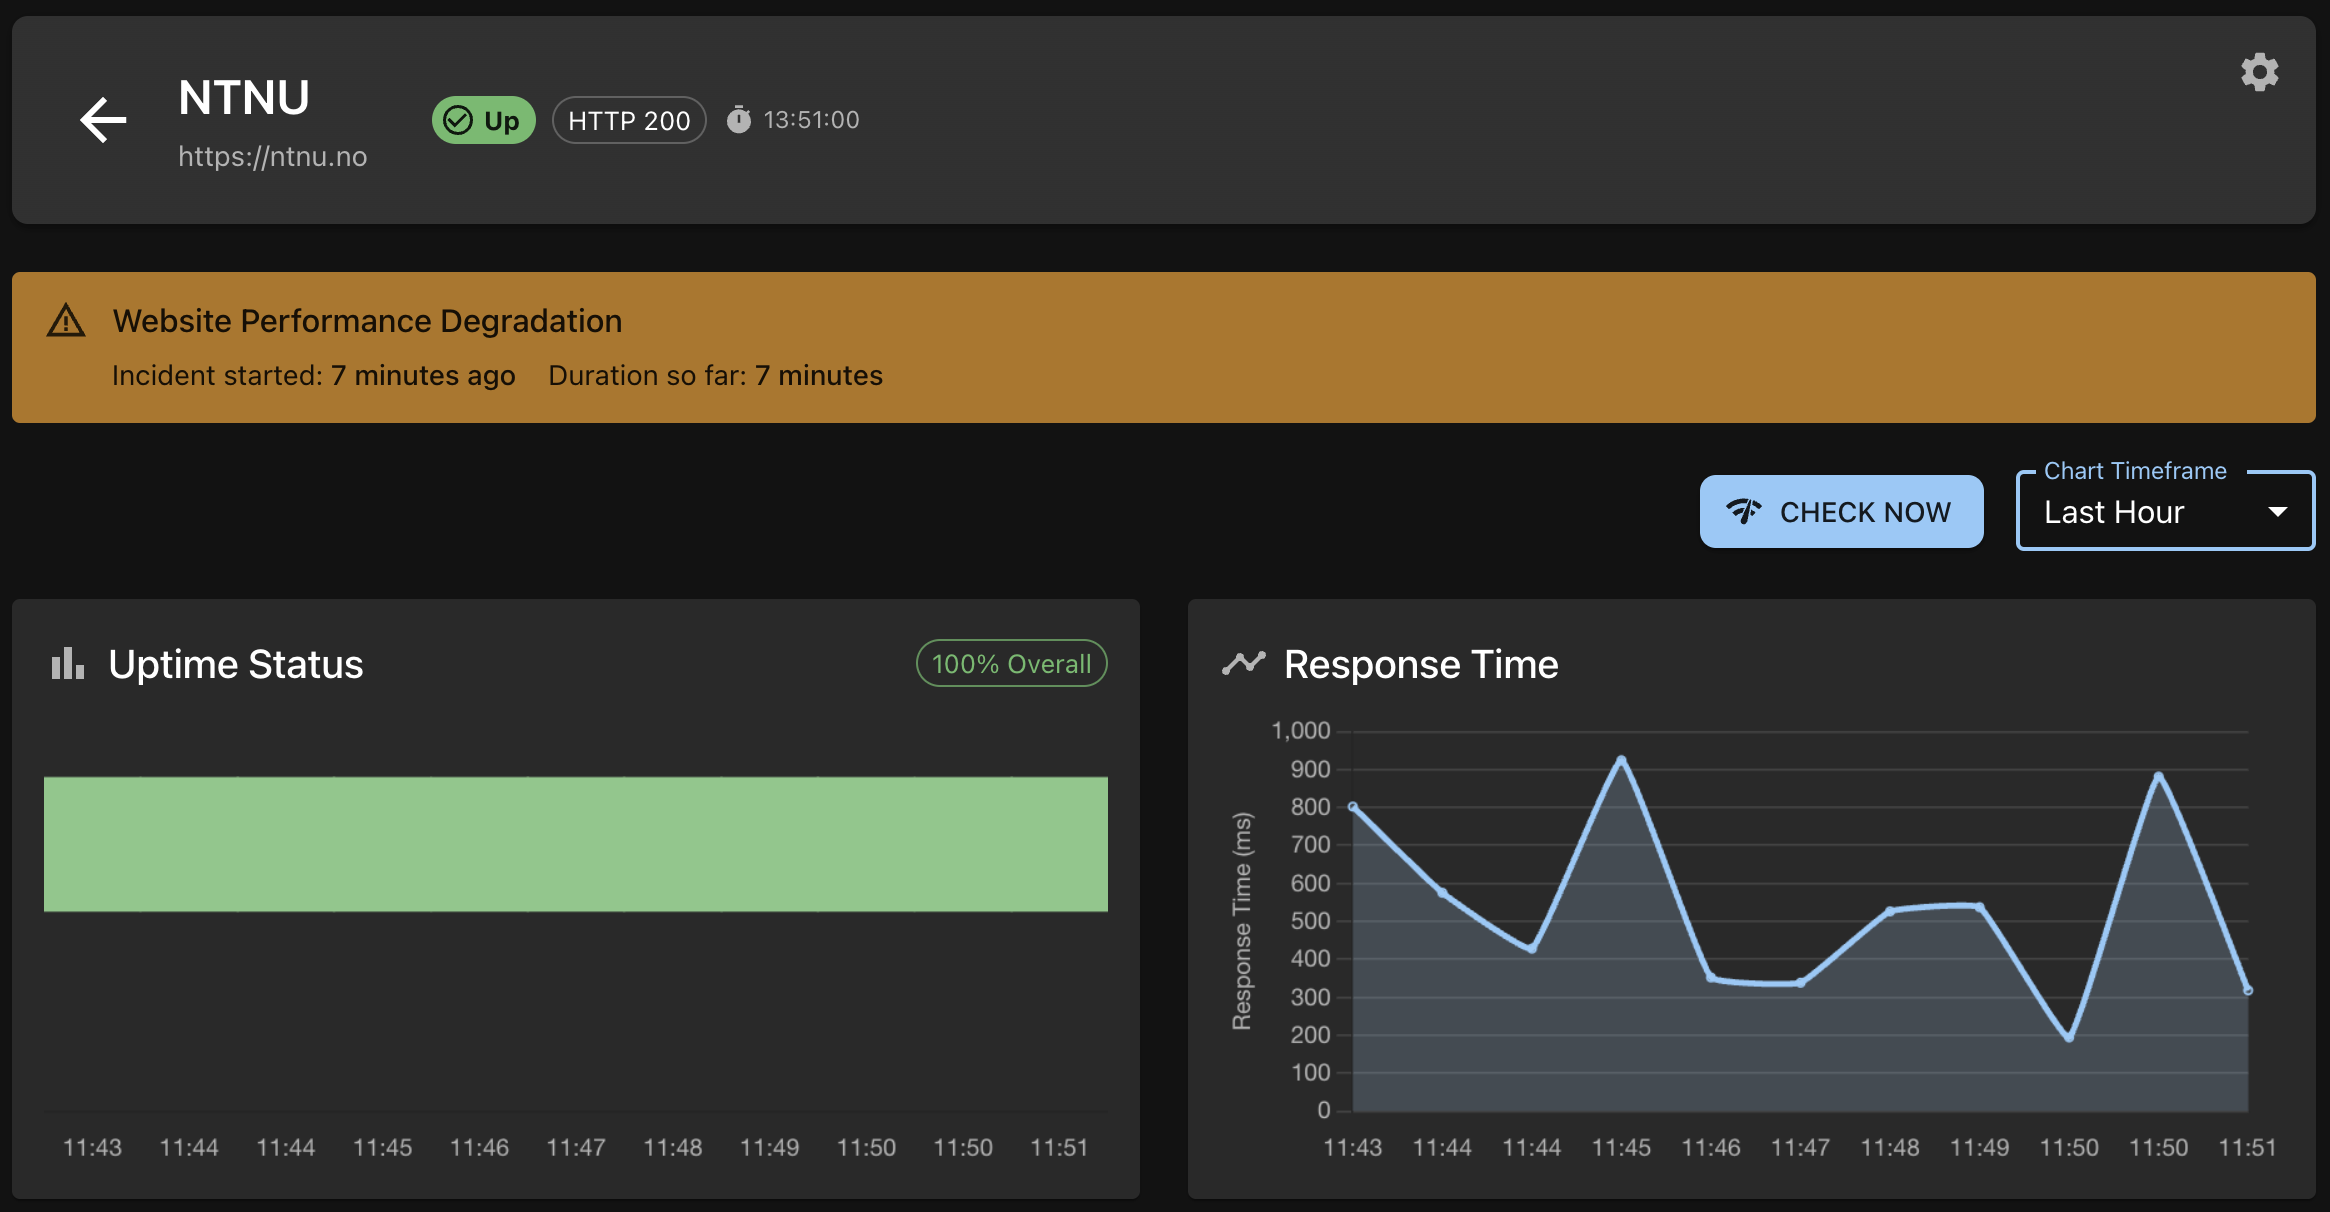
\includegraphics[width=1\linewidth]{figures/websiteDetails.png}
    \caption{Enter Caption}
    \label{fig:enter-label}
\end{figure}


\begin{figure}[H]
    \centering
    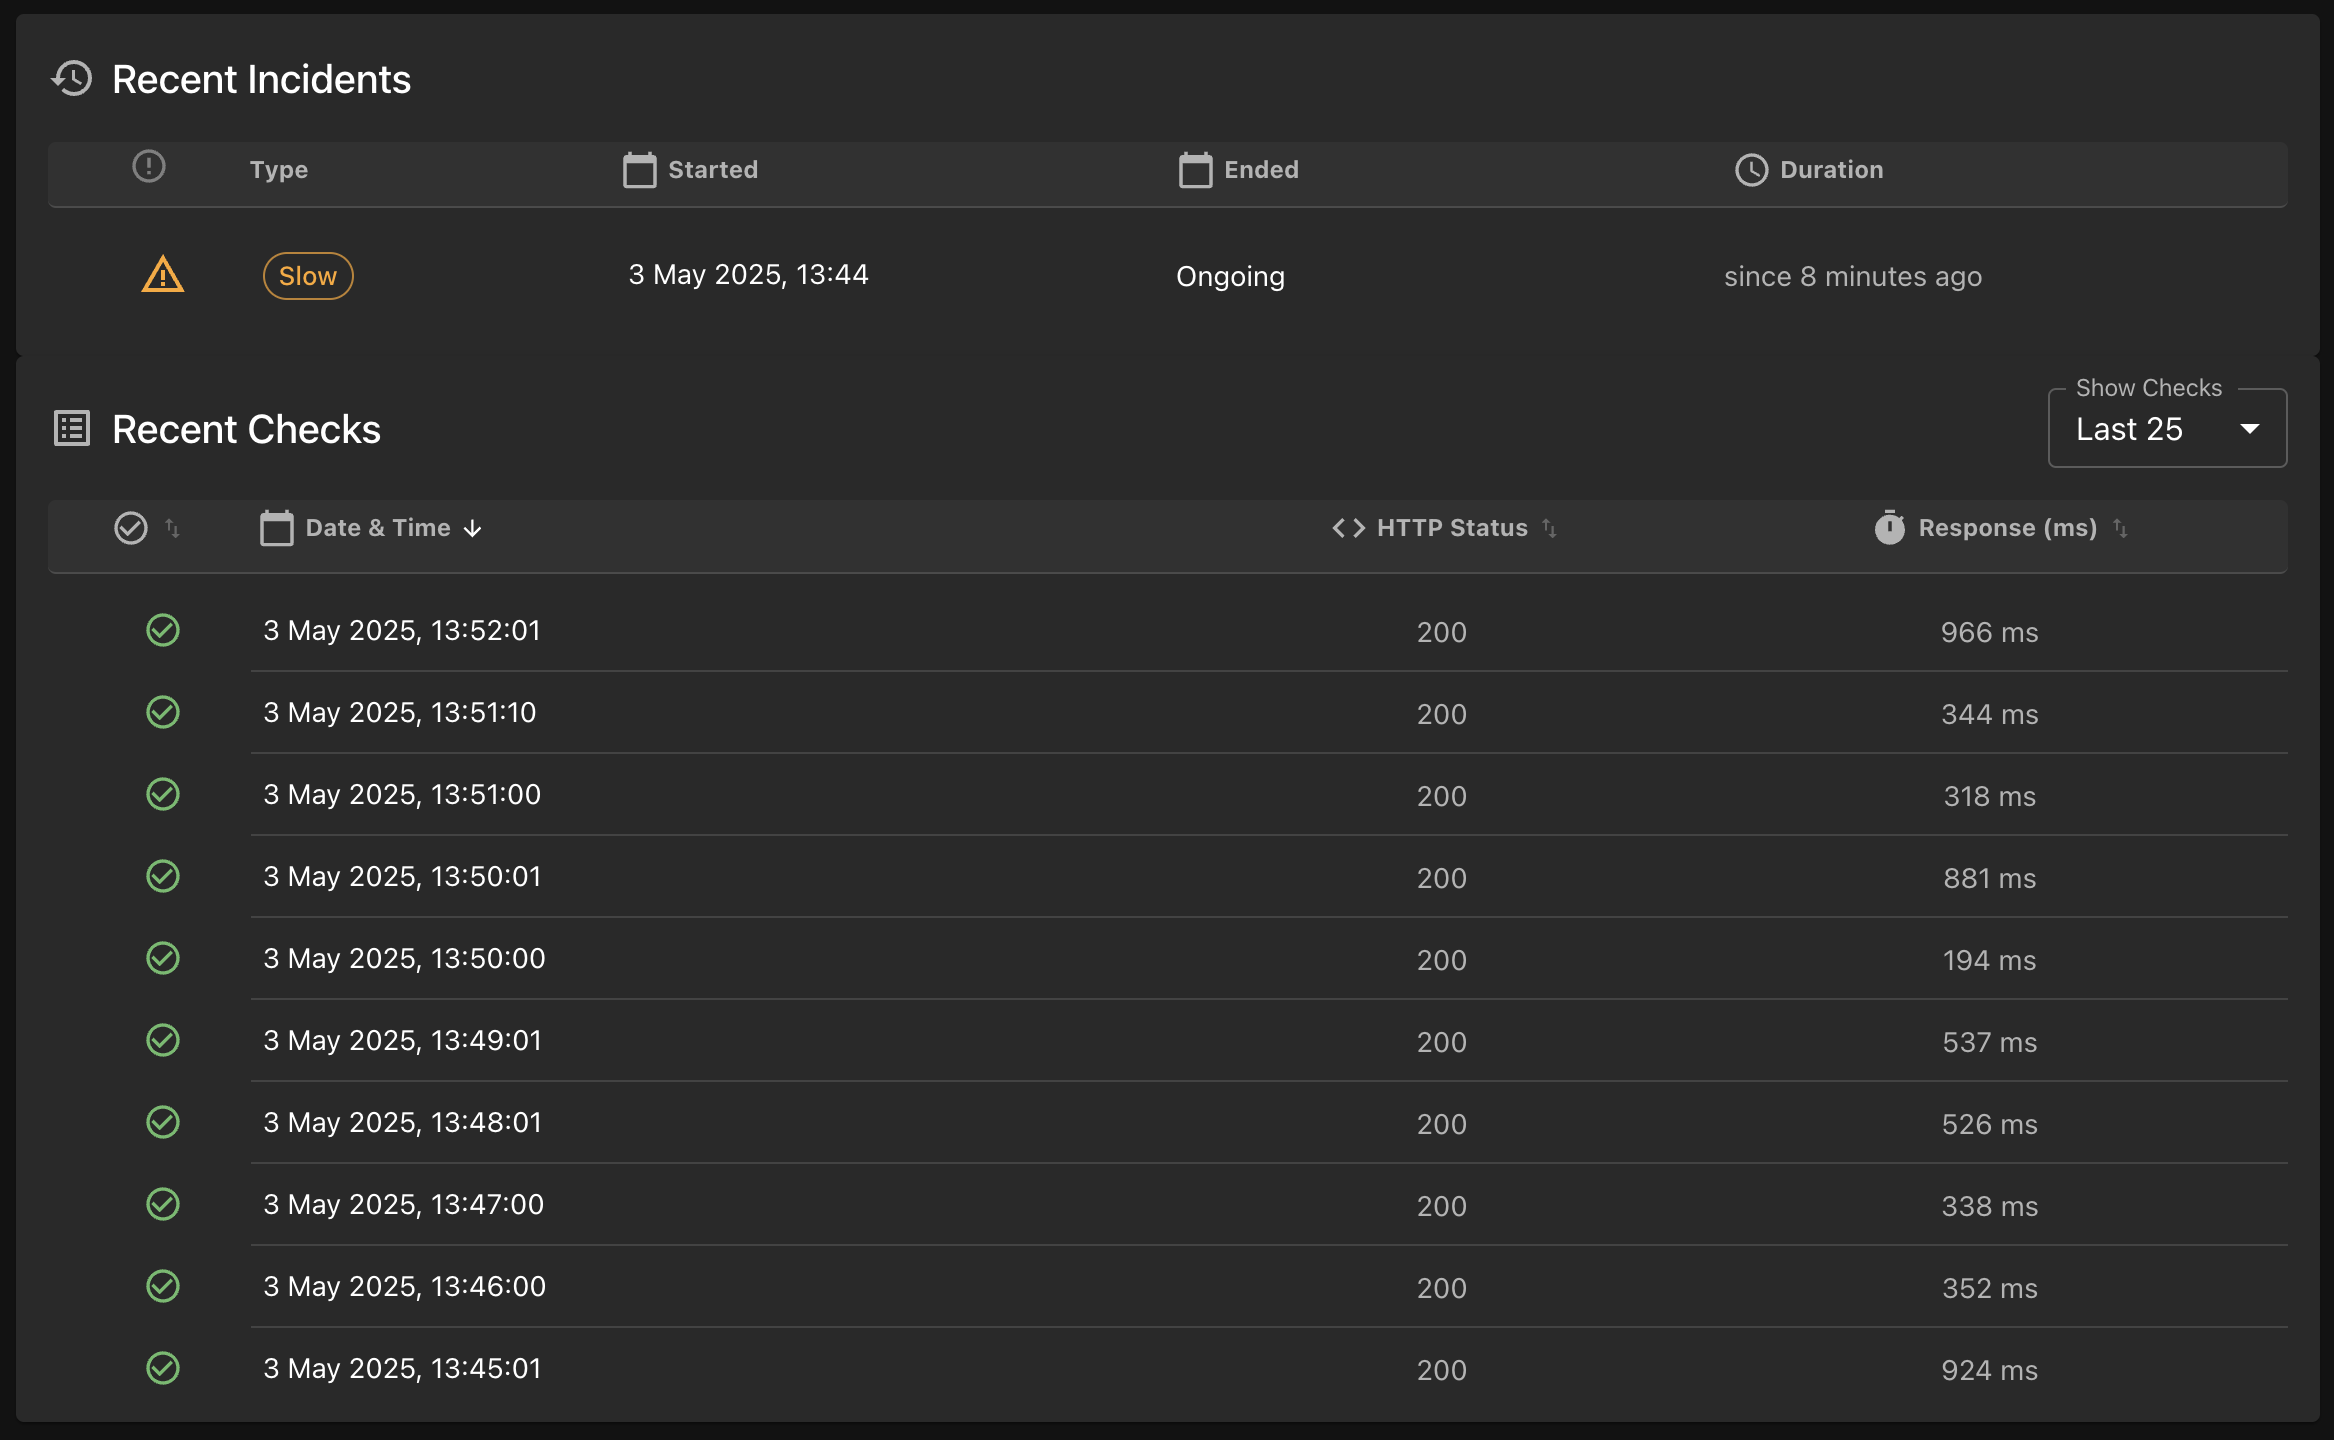
\includegraphics[width=1\linewidth]{figures/websiteDetails_bottom.png}
    \caption{Enter Caption}
    \label{fig:enter-label}
\end{figure}


%diskutere om disse her faktisk skal tas med I forhold til designvalg
\subsubsection{Incident list component}



\subsection{Requirement Fulfillment}

The application fulfilled nearly all high-priority functional and non-functional requirements from Tables~\ref{tab:functional_reqs_refined} and~\ref{tab:nonfunctional_reqs_refined}:

\begin{itemize}
    \item \textbf{Fully fulfilled:} F.1–F.4, F.6–F.8, NF.1–NF.3.
    \item \textbf{Partially fulfilled:} 
        \begin{itemize}
            \item F.5 – User authentication was implemented, but support for multi-role access (e.g., admin vs. viewer) was not.
            \item F.9 – Users can adjust check intervals, but the server does not enforce hard limits.
            \item NF.4 – The codebase is documented, but not extensively.
        \end{itemize}
    \item \textbf{Not implemented:} NF.5 – The system layout is responsive, but mobile-specific testing and optimizations were limited.
\end{itemize}

An additional requirement, F.11, was introduced during testing to track website incidents. This feature was implemented successfully and provided additional clarity for users.


intill videre idk if skal være her:

\subsection{ER Diagram / Domain Model}
\begin{figure}[H]
        \centering
        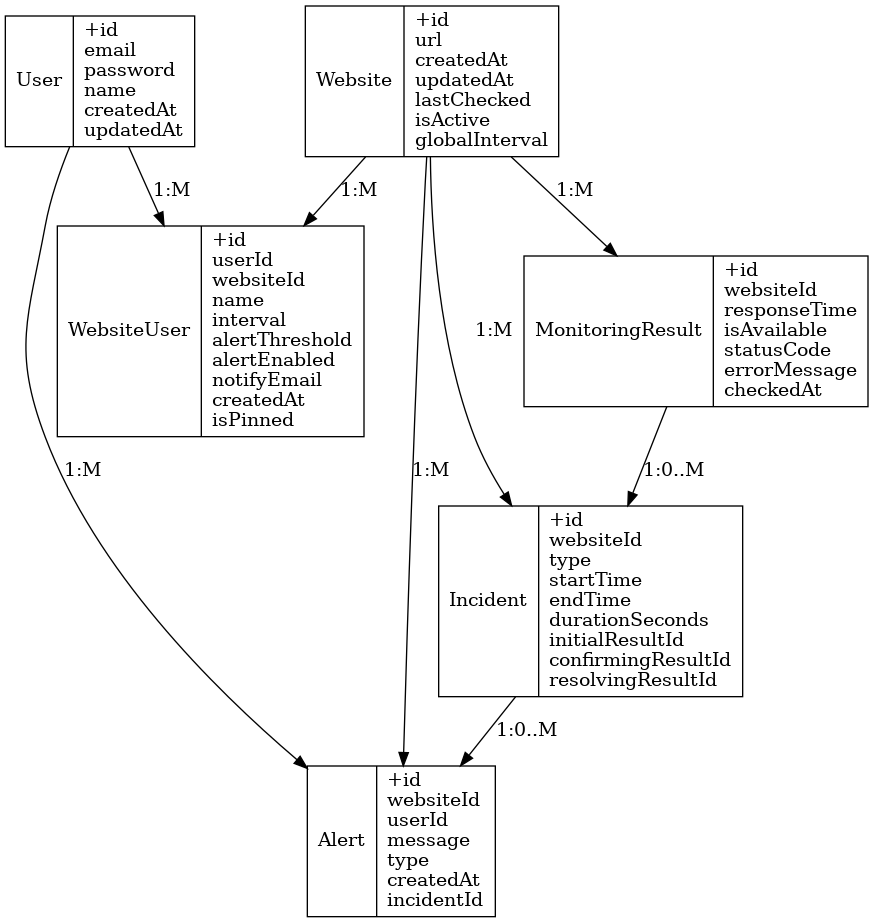
\includegraphics[width=\textwidth]{figures/ER_diagram.png}
        \caption{Entity Relations Diagram}
        \label{sfig:er_diagram}
\end{figure}

\begin{figure}[H]
        \centering
        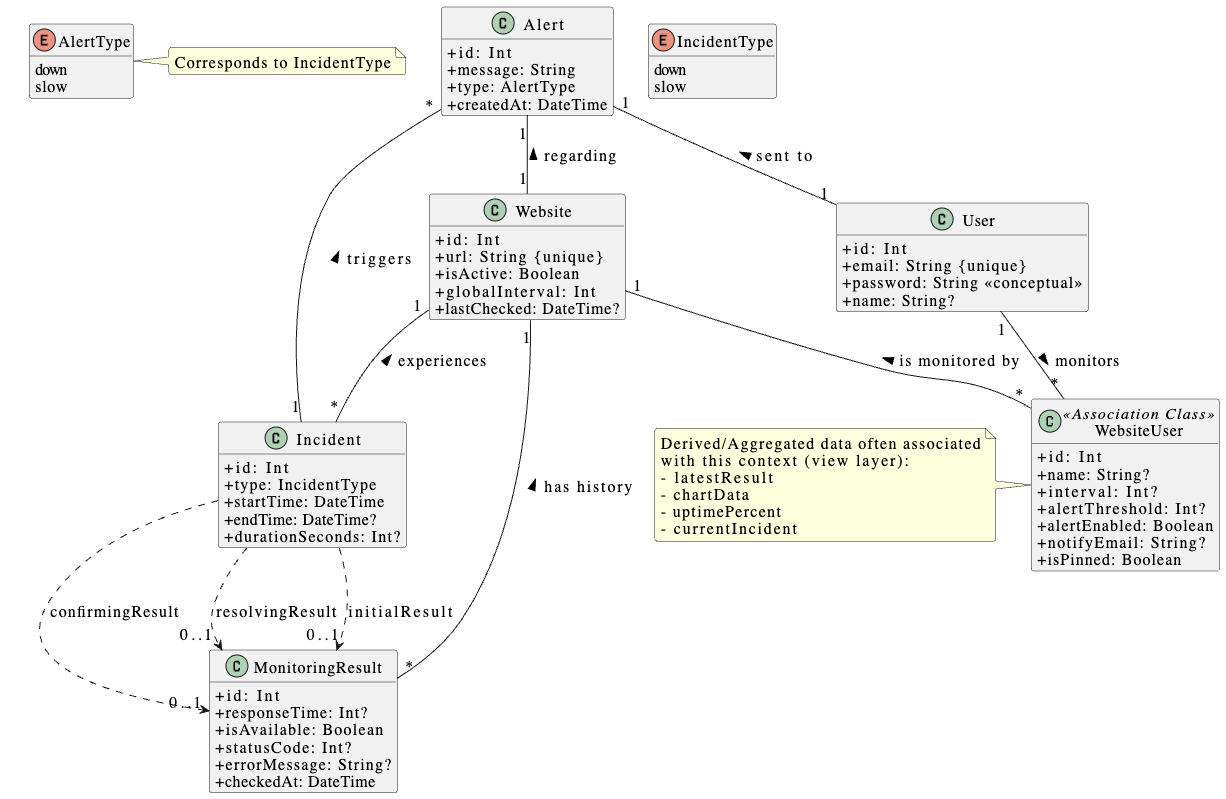
\includegraphics[width=\textwidth]{figures/domainmodel.png}
        \caption{Domain Model}
        \label{sfig:domain_model}
\end{figure}


\section{Summary of Development Process} 
This chapter described how user and stakeholder needs were translated into a working monitoring system through iterative development, prototyping, testing, and refinement. The technology stack, implementation strategies, and evaluation results collectively demonstrate a system that meets most core requirements and reflects key principles of usability, maintainability, and responsiveness.